\subsection{Regular expression to NFA}
\label{sec:from_regular_expression_to_nfa}
Every regular expressions can be converted to a NFA matching the same
language.  This section will describe an approach to doing so.

\subsubsection{Thompson}
\label{sec:re2nfa_thompson_theory}
The method described in this section first appeared in Ken Thompsons
article from 1968 \cite{Thompson1968}. The descriptions given in for
example \cite{HopcroftJohnE.AndMotwaniRajeevAndUllman2001},
\cite{Aho:1986:CPT:6448} and \cite{RussCox} are considered more
readable and we will be basing our description on these.

The NFA will be build in steps from smaller NFA fragments. A NFA
fragment has an initial state, but no accepting state, instead it has
one or more dangling edges leading nowhere (yet).


%% a method for converting a
%% regular expression to an automaton is described. The method works by
%% breaking the regular expression up into fragments; Each fragment also
%% being a regular expression in itself. Using this method yields an
%% automaton with the following characteristics:
%% \begin{itemize}
%% \item There is exactly one initial state
%% \item There are no edges into the initial state
%% \item There is exatly one accepting state
%% \item There are no edges out of the accepting state
%% \item There are at most two edges leaving a state
%% \end{itemize}

The base fragment corresponds to the regular expression consisting
only of a single character \textit{a}. The NFA fragment is shown in
figure \vref{fig:basecase1}. One state with a single edge, marked with
the character \textit{a} is added. The new state is the initial state
for this fragment and the edge is left dangling.

\begin{figure}
  \centering
  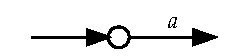
\includegraphics{parsing/basecase1}
  \caption{Fragment accepting a single character \textit{a}}
  \label{fig:basecase1}
\end{figure}

The second base fragment corresponds to the empty regular
expression. The NFA fragment is shown in figure
\vref{fig:basecase4}. One state with a single edge marked as a
$\upvarepsilon$-edge is added. The new state is the initial state for
this fragment and the edge is left dangling. This fragment is used for
the empty regular expression and for alternations with one or more
options left empty.

%% In Ken Thompson article from 1968 \cite{Thompson1968}, in
%% \cite{HopcroftJohnE.AndMotwaniRajeevAndUllman2001} and in
%% \cite{RussCox} a method for converting a regular expression to an
%% automaton is described.



%% The base case is the regular expression consisting of a single
%% character \textit{a}. Figure \vref{fig:basecase1} shows an automaton
%% accepting the same language. 

\begin{figure}
  \centering
  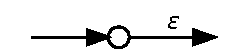
\includegraphics{parsing/basecase4}
  \caption{Fragment accepting the empty string}
  \label{fig:basecase4}
\end{figure}


%% \begin{figure}
%%   \centering
%%   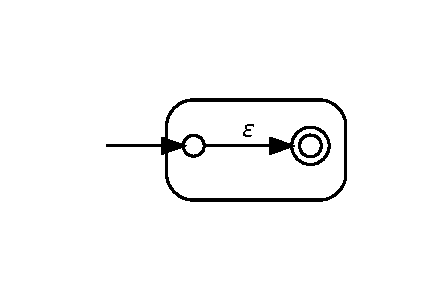
\includegraphics{parsing/basecase3}
%%   \caption{The empty string}
%%   \label{fig:basecase3}
%% \end{figure}

The first compound fragment is alternation, see figure
\vref{fig:alternation}. Here, the two sub-fragments R and S are automatons
with initial states and some dangling edges. What else they are
composed of, is irrelevant for the moment\todo{changed}. We add one new state, 
and make it the initial state for this fragment. The initial state has two
$\upvarepsilon$-edges leaving, connecting to the initial states of R
and S. The dangling edges for the new fragment is the sum of the
dangling edges leaving R and S.

\begin{figure}
  \centering
  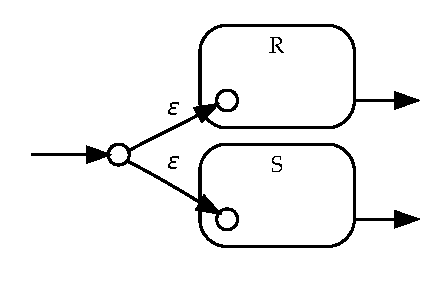
\includegraphics{parsing/alternation}
  \caption{Alternation R\textbar S}
  \label{fig:alternation}
\end{figure}

Concatenation of two regular expressions R and S is achieved as shown
in figure \vref{fig:concatenation}. The dangling edges of R is
connected to the initial state of S. The initial state for the new
fragment is the initial state of R and the dangling edges of S is
still left dangling.

\begin{figure}
  \centering
  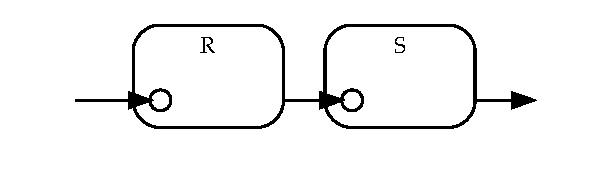
\includegraphics{parsing/concatenation}
  \caption{Concatenation RS}
  \label{fig:concatenation}
\end{figure}

Zero or more times repetition is shown in figure
\vref{fig:repetition}. One new, initial, state is added. It has two
$\upvarepsilon$-edges leaving, one is connected to the initial state of
R and one is left dangling. The dangling edges of R is connected to
the new initial state.

\begin{figure}
  \centering
  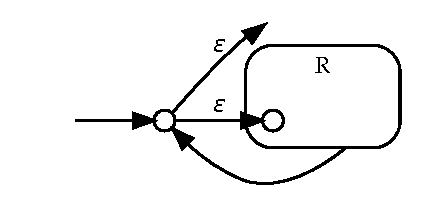
\includegraphics{parsing/repetition}
  \caption{Repetition R*}
  \label{fig:repetition}
\end{figure}

Finally an accepting state is patched into the NFA. All edges left
dangling is connected to the accepting state. 

\paragraph{Properties} NFAs created with Thompsons method has these
properties:
\begin{itemize}
  \item At most two edges is leaving a state
  \item There are no edges leaving the accepting state
  \item There are no edges leading into the starting state
\end{itemize}


\begin{example}[Converting a regular expression to a NFA]
\label{ex:converting_a_regular_expression_to_a_nfa}
\begin{figure}
  \centering 
  \subfigure[Fragment for \textsf{a}]{
    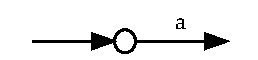
\includegraphics{parsing/ex_a.pdf}
    \label{fig:ex_parsing_a}
  }
  \subfigure[Fragment for \textsf{b}]{
    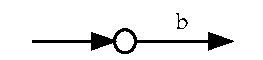
\includegraphics{parsing/ex_b.pdf}
    \label{fig:ex_parsing_b}
  }
  \subfigure[Fragment for \textsf{c}]{
    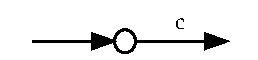
\includegraphics{parsing/ex_c.pdf}
    \label{fig:ex_parsing_c}
  }
  \subfigure[Fragment for \textsf{a*}]{
    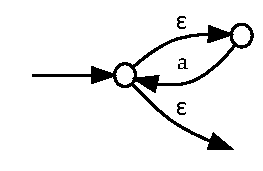
\includegraphics{parsing/ex_star.pdf}
    \label{fig:ex_parsing_star}
  }
  \subfigure[Fragment for \textsf{a*b}]{
    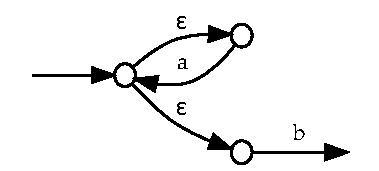
\includegraphics{parsing/ex_concat.pdf}
    \label{fig:ex_parsing_concat}
  }
  \subfigure[Fragment for \textsf{a*b\textbar c}]{
    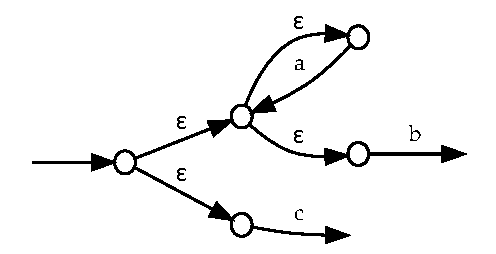
\includegraphics{parsing/ex_alt.pdf}
    \label{fig:ex_parsing_alt}
  }
  \subfigure[Final NFA for \textsf{a*b\textbar c}]{
  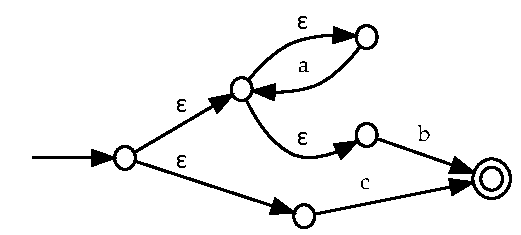
\includegraphics{parsing/ex_finished.pdf}
  \label{fig:ex_parsing_finished}
  }
  \caption{Individual fragments when converting \textsf{a*b\textbar c}
    to NFA}
  \label{fig:ex_parsing}
\end{figure}

\begin{figure}
\end{figure}


In this example we will be converting the regular expression
\textsf{a*b\textbar c} to a NFA using Thompsons method.
\begin{itemize}
\item Top level we have the alternation operator, but before we can
  complete this fragment, we need to convert \textsf{a*b} and
  \textsf{c} to fragments.
  \begin{itemize}
  \item \textsf{a*b} is complicated since we have one operator, two
    literals and a hidden concatenation. Top level we have the
    concatenation operator, concatenating \textsf{a*} and
    \textsf{b}. These needs to be converted before we can concatenate.
    \begin{itemize}
    \item \textsf{a*} needs to be broken further down. Top level we have
      the Kleene star, but we can not apply the rule for converting this
      to a NFA fragment before we have converted \textsf{a}. 
      \begin{itemize}
        \item \textsf{a} is straightforward, we just apply the rule
          for transforming literals and we have the fragment in figure
          \ref{fig:ex_parsing_a}
      \end{itemize}
      Using this fragment to complete the Kleene star, we have the
      fragment in figure \ref{fig:ex_parsing_star}.
    \item \textsf{b} is straightforward, we just apply the rule for
      transforming literals and we have the fragment in figure
      \ref{fig:ex_parsing_b}.
    \end{itemize}
    Now we are ready to concatenate, fragments
    \ref{fig:ex_parsing_star} and \ref{fig:ex_parsing_b} are
    concatenated and we have the fragment in figure \ref{fig:ex_parsing_concat}
  \item \textsf{c} is straightforward, we just apply the rule for
    transforming literals and we have the fragment in figure
    \ref{fig:ex_parsing_c}.
  \end{itemize}
  With these expressions converted to fragments we can apply the
  alternation conversion rule. We have the resulting fragment in
  figure \ref{fig:ex_parsing_alt}
\end{itemize}

All that is left now is to connect the dangling edges to an accepting
state. We have the final result in figure \vref{fig:ex_parsing_finished}
  
\end{example}

\subsection{Matching}

The NFAs constructed as described in section
\vref{sec:from_regular_expression_to_nfa} can be used to match a
regular expression with a string, i.e. to determine if a string belongs
to the language of the regular expression. 

Once the NFA is generated, simulating it is a straightforward
task. Again, our method is attributed to Thompson
\cite{Thompson1968}. 
\begin{enumerate}
    \item We maintain a set of active states and a pointer
    to the current character in the string
    \item At the beginning only the
    start state belongs to the set of active states
    \item The string is read
    from left to right, taking each character in turn. When a character is
    read from the input string, all legal transitions from the states in
    the active set is followed
    \item A transition is legal if it is a
    $\upvarepsilon$-transition or if the mark on the transition matches
    the character read from the input string. The new set of active states
    is the set of end states for the transitions followed
    \item If the
    accepting state is included in the active set when the string is read,
    the string matches the regular expression
\end{itemize}

With this method we only ever add a state to the active set once per
iteration and we only read each character from the input string once.


\begin{example}[Matching with a NFA]
  \begin{figure}
    \centering
    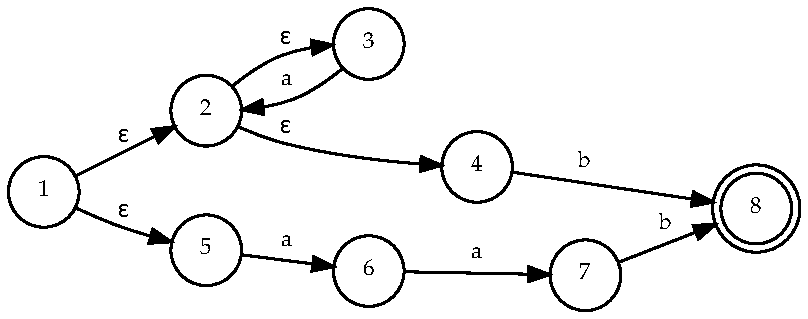
\includegraphics[width=\textwidth]{matching/ex_matching.pdf}
    \caption{NFA for the regular expression \textsf{a*b\textbar aab}}
    \label{fig:ex_matching}
  \end{figure}
  
  In this example we will demonstrate how the regular expression
  \textsf{a*b\textbar aab} is matched with the string \textsl{aab}. In
  figure \vref{fig:ex_matching} we have the corresponding NFA. Each
  state is marked with a unique number which we will be referring to
  in the table below.

\begin{center}
\begin{tabular}{ccp{8.5cm}}
Active set & \texttt{SP} & Explanation \\
\hline

1 & \textsl{\underline{a}ab} & Initially we have the start state in
the active set and \texttt{SP} points to the start of the string. \\

3, 4, 5 & \textsl{\underline{a}ab} & Following all
$\upvarepsilon$-transitions. \\

2, 6 & \textsl{a\underline{a}b} & Reading the first \textsl{a} from the input
string, states 3 and 5 have legal transitions on \textsl{a}. \\

3, 4, 6 & \textsl{a\underline{a}b} & Following all
$\upvarepsilon$-transitions. \\

2, 7 & \textsl{aa\underline{b}} & Reading the second \textsl{a} from
the input string, states 3 and 6 have legal transitions on
\textsl{a}. \\

3, 4, 6 & \textsl{aa\underline{b}} & Following all
$\upvarepsilon$-transitions. \\

8 & \textsl{aab\underline{ }} & Reading the last character from input
string: \textsl{b}, states 4 and 7 have legal transitions on
\textsl{b}. \\

8 & \textsl{aab\underline{ }} & No $\upvarepsilon$-transitions to follow.

\end{tabular}
\end{center}

After reading the string we can see that the accepting state is in the
active set: We have a match!

\end{example}

